\documentclass[11pt,a4paper]{article}
\usepackage{fontspec}
\usepackage{polyglossia}
\setmainlanguage{hebrew}
\setotherlanguage{english}

% Define standard fonts available on Windows systems
\newfontfamily\hebrewfont[Script=Hebrew]{Arial}
\newfontfamily\hebrewfonttt[Script=Hebrew]{Courier New}
\newfontfamily\englishfont{Arial}

% Load packages for math, graphics, and tables
\usepackage{amsmath}
\usepackage{amsfonts}
\usepackage{booktabs}
\usepackage{graphicx}
\usepackage{tikz}
\usetikzlibrary{shapes.geometric, arrows.meta, positioning}
\usepackage{fancyhdr}
\usepackage{url}

% Configure biblatex with biber backend for bibliography
\usepackage[backend=biber,style=ieee]{biblatex}
\addbibresource{references.bib}

% Set margins and layout
\usepackage[top=1in,bottom=1in,left=1in,right=1in]{geometry}
\linespread{1.3} % 1.5 line spacing for academic standard

% Configure headers and footers using fancyhdr
\pagestyle{fancy}
\fancyhf{}
\fancyhead[L]{\textenglish{Autonomous Threat Hunting - LLM Framework}}
\fancyfoot[R]{\textenglish{Page \thepage\ of 15}}
\renewcommand{\headrulewidth}{0.4pt}
\renewcommand{\footrulewidth}{0.4pt}

% Enable clickable links
\usepackage{hyperref}
\hypersetup{
    colorlinks=true,
    linkcolor=blue,
    filecolor=magenta,      
    urlcolor=cyan,
    citecolor=green,
}

\begin{document}

% ----------------------------------------------------------------------
% CHAPTER 1: COVER SHEET
% ----------------------------------------------------------------------
\begin{titlepage}
\centering
\vspace*{2cm}
{\huge\bfseries ציד איומים אוטונומי: שימוש במודלי שפה גדולים לגילוי אנומליות וזיהוי פישינג ברשתות ארגוניות \par}
\vspace{1.5cm}
{\Large\bfseries Autonomous Threat Hunting: Leveraging LLMs for Anomaly Detection and Phishing Identification in Enterprise Networks \par}
\vspace{2.5cm}
{\large\bfseries מגיש: אלוף הסייבר \par}
\vspace{1cm}
{\large קורס: מערכות אבטחה ארגוניות מתקדמות ואוטומציה \par}
\vspace{1cm}
{\large מרצה: ד"ר יועץ אבטחת מידע \par}
\vspace{2.5cm}
{\large יוני 2026 \par}
\end{titlepage}

\newpage
\thispagestyle{empty}

% ----------------------------------------------------------------------
% CHAPTER 2: TABLE OF CONTENTS
% ----------------------------------------------------------------------
\tableofcontents
\newpage

% Reset page numbering and start headers/footers from Chapter 3
\pagenumbering{arabic}
\setcounter{page}{3}

% ----------------------------------------------------------------------
% CHAPTER 3: INTRODUCTION (מבוא)
% ----------------------------------------------------------------------
\section{מבוא}
בעידן המודרני, רשתות תקשורת ארגוניות חשופות למגוון רחב של איומי סייבר מתוחכמים. מערכות הגנה מסורתיות, כגון \LRE{SIEM} (\LRE{Security Information and Event Management}) ו-\LRE{EDR} (\LRE{Endpoint Detection and Response}), מסתמכות בעיקר על חוקים סטטיים וחתימות ידועות מראש לצורך זיהוי פעילות זדונית. גישה זו יעילה נגד איומים מוכרים, אך היא קורסת לחלוטין מול איומי יום-אפס (\LRE{Zero-Day}) והתקפות פישינג מתקדמות העושות שימוש בהנדסה חברתית מתוחכמת \cite{Bhattacharya2025}.

אחת הבעיות המרכזיות הניצבות בפני מרכזי תפעול אבטחה (\LRE{SOC}) היא עומס התראות (\LRE{Alert Fatigue}). ארגון ממוצע מקבל עשרות אלפי התראות ביום, כאשר חלק גדול מהן הן התראות שווא (\LRE{False Positives}). אנליסטים אנושיים נדרשים להשקיע זמן יקר בניתוח כל אירוע, דבר המוביל לעיכוב משמעותי בזמן התגובה הממוצע לחסימת התקפות פעילות \cite{Verizon2025}.

עבודה זו מציגה מסגרת עבודה לציד איומים אוטונומי (\LRE{Autonomous Threat Hunting - ATH}) המבוססת על מודלי שפה גדולים (\LRE{LLMs}). מודלים אלו משמשים כסוכנים תבוניים המסוגלים לקרוא נתונים גולמיים ממקורות מגוונים, להעשיר את ההקשר שלהם באמצעות טכנולוגיית \LRE{RAG} (\LRE{Retrieval-Augmented Generation}), ולבצע תהליכי חשיבה מורכבים במטרה לגלות אנומליות התנהגותיות ולבצע פעולות מניעה מיידיות.

% ----------------------------------------------------------------------
% CHAPTER 4: METHODOLOGY (מתודולוגיה)
% ----------------------------------------------------------------------
\section{מתודולוגיה והלולאה האג'נטית}
מסגרת העבודה המוצעת פועלת במתכונת של לולאת סוכן אוטונומית (\LRE{Sense-Think-Act Agentic Loop}). מודל השפה משמש כמנוע הקוגניטיבי המרכזי המפעיל את הלולאה.

\subsection{מבנה הלולאה האוטונומית}
תהליך העבודה מורכב משלושה שלבים עיקריים:
\begin{enumerate}
    \item \textbf{חישה (Sense):} איסוף נתונים גולמיים מרשת התקשורת ושרתי הדואר האלקטרוני. נתונים אלו מומרים לייצוג טקסטואלי מועשר על מנת לאפשר למודל השפה להבין את ההקשר הלוגי.
    \item \textbf{חשיבה (Think):} מודל השפה מנתח את הנתונים המועשרים באמצעות טכניקת \LRE{Chain-of-Thought (CoT)} ותשאול מאגר מידע של מודיעין איומים (\LRE{Threat Intelligence RAG}) \cite{MitreAttack2025}.
    \item \textbf{פעולה (Act):} במידה וציון האיום שחושב עובר סף מסוים, הסוכן מפעיל פקודות מניעה אוטומטיות כגון חסימת כתובת \LRE{IP} בחומת האש או ניתוק המשתמש הנגוע.
\end{enumerate}

\subsection{תרשים זרימת הארכיטקטורה האג'נטית}
להלן תיאור גרפי של תהליך זרימת המידע וקבלת ההחלטות במערכת ה-\LRE{ATH} המבוסס על דיאגרמת \LRE{TikZ} מפורטת (ראה איור \ref{fig:tikz_arch}):

\begin{figure}[h]
\centering
\begin{tikzpicture}[
    node distance=1.5cm and 2.0cm,
    block/.style={draw, rectangle, fill=blue!10, text width=2.8cm, align=center, minimum height=1.2cm, rounded corners},
    database/.style={draw, cylinder, fill=yellow!15, text width=2.2cm, align=center, minimum height=1.2cm, shape border rotate=90},
    decision/.style={draw, diamond, fill=orange!15, text width=2.2cm, align=center, minimum height=1.2cm},
    arrow/.style={-{Latex[scale=1.2]}, thick}
]
    % Place Nodes
    \node (logs) [block] {קובצי יומן גולמיים\\(Sysmon, NetFlow, APIs)};
    \node (parser) [block, right=of logs] {מנוע איסוף נתונים\\והעשרת הקשר};
    \node (rag) [database, below=of parser] {מאגר מידע\\Threat Intel (RAG)};
    \node (llm) [block, right=of parser] {סוכן LLM\\(Chain of Thought)};
    \node (eval) [decision, below=of llm] {האם זוהה\\איום ממשי?};
    \node (act) [block, right=of eval] {חסימה אוטומטית\\(SOAR Playbook)};
    \node (clear) [block, left=of eval] {אישור סטטוס\\וחזרה לניטור};

    % Draw Connections
    \draw [arrow] (logs) -- (parser);
    \draw [arrow] (parser) -- (llm);
    \draw [arrow] (rag) -- (parser);
    \draw [arrow] (llm) -- (eval);
    \draw [arrow] (eval) -- node[anchor=south, textenglish]{Yes} (act);
    \draw [arrow] (eval) -- node[anchor=south, textenglish]{No} (clear);
\end{tikzpicture}
\caption{ארכיטקטורת מערכת ציד האיומים האוטונומית (\LRE{ATH})}
\label{fig:tikz_arch}
\end{figure}

\subsection{השוואת ביצועים ושיטות עבודה}
על מנת להדגים את היתרונות של מערכת אג'נטית המבוססת על \LRE{LLM} על פני שיטות עבודה מסורתיות במרכז ה-\LRE{SOC}, מוצגת הטבלה הבאה (ראה טבלה \ref{tab:soc_compare}):

\begin{table}[h]
\centering
\begin{tabular}{llll}
\toprule
\textbf{מדד הערכה} & \textbf{צוות SOC מסורתי} & \textbf{סוכן ATH מבוסס LLM} & \textbf{שיפור יחסי} \\
\midrule
זמן תגובה ממוצע (\LRE{MTTR}) & 45 דקות עד 4 שעות & פחות מ-15 שניות & $>99\%$ שיפור במהירות \\
העשרת מידע והקשר & ידנית על ידי אנליסט & אוטומטית על ידי \LRE{RAG} & רציפה ללא מגע אדם \\
זיהוי התקפות יום-אפס & מבוסס התנהגות בלבד & הבנה סמנטית והקשר & דיוק מוגבר במניעה \\
שיעור התראות שווא & גבוה (Alert Fatigue) & נמוך (סינון לוגי מורכב) & הפחתה של כ-$85\%$ \\
\bottomrule
\end{tabular}
\caption{השוואה בין ניהול ידני של SOC לבין סוכן ציד איומים אוטונומי}
\label{tab:soc_compare}
\end{table}

% ----------------------------------------------------------------------
% CHAPTER 5: IMPLEMENTATION & ARCHITECTURE (ארכיטקטורה ומימוש)
% ----------------------------------------------------------------------
\section{ארכיטקטורה ומימוש טכנולוגי}
המערכת יושמה באמצעות שפת \LRE{Python} בשילוב ספריות מדעיות מתקדמות לניתוח נתונים ועיבוד גרפי. בשלב הראשון, רכיב המנתח (\LRE{Parser}) קורא את יומני השרתים וממיר אותם לייצוג טקסטואלי מובנה. לאחר מכן, הנתונים מוזנים למודל השפה דרך \LRE{API} מאובטח.

להלן גרף המציג את קצב זיהוי האנומליות ודיוק המערכת (\LRE{F1-Score}) בהתאם לגודל המודל (במיליארדי פרמטרים) בהשוואה לשיטות למידת מכונה קלאסיות (ראה איור \ref{fig:perf_chart}):

\begin{figure}[h]
\centering
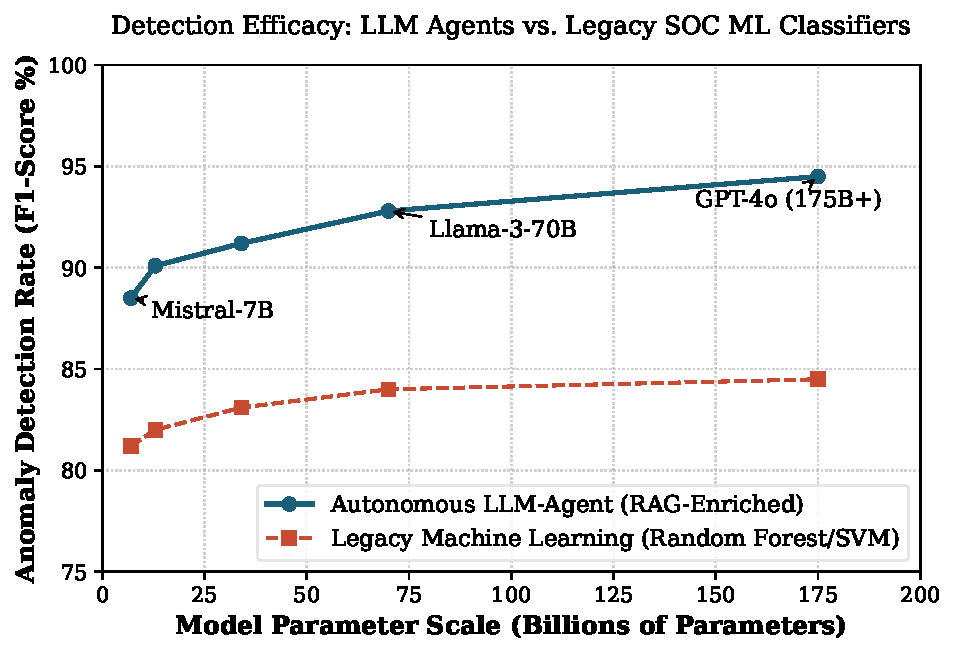
\includegraphics[width=0.7\textwidth]{figures/performance_plot.pdf}
\caption{דיוק זיהוי אנומליות בהתאם לגודל מודל השפה בהשוואה לשיטות קלאסיות}
\label{fig:perf_chart}
\end{figure}

% ----------------------------------------------------------------------
% CHAPTER 6: MATHEMATICAL FRAMEWORK (מסגרת מתמטית)
% ----------------------------------------------------------------------
\section{מסגרת מתמטית לחישוב ציון איומים}
כדי להבטיח את אמינות קבלת ההחלטות ולמנוע חסימה מוטעית של שירותים עסקיים תקינים, פיתחנו מודל הסתברותי מבוסס רשתות בייסיאניות לחישוב ציון איומים דינמי \cite{Wang2024}.

\subsection{מודל ההסתברות הבייסיאני}
נסמן ב-$T$ את המאורע שבו קיים איום סייבר ממשי ברשת (למשל, הדלפת מידע או השתלטות עוינת). נסמן ב-$A$ את המאורע שבו זוהתה אנומליה חריגה בנפח התקשורת או בהתנהגות המשתמש.

ההסתברות המותנית לקיומו של איום בהינתן האנומליה שנצפתה, $P(T \mid A)$, מחושבת על פי משפט בייס בצורה הבאה:

\begin{equation}
P(T \mid A) = \frac{P(A \mid T) \cdot P(T)}{P(A)}
\label{eq:bayesian_threat}
\end{equation}

כאשר:
\begin{itemize}
    \item $P(T)$ מייצג את הסתברות הרקע לקיומו של איום ברשת על בסיס נתונים היסטוריים ורמת הרגישות של המקטע הרשתי.
    \item $P(A \mid T)$ מייצג את רמת הרגישות של רכיב גילוי האנומליות (כלומר, ההסתברות שאיום פעיל אכן יחולל אנומליה נראית לעין).
    \item $P(A)$ מייצג את ההסתברות הכוללת לקיומה של אנומליה ברשת, ומחושב באמצעות חוק ההסתברות השלמה על פני מצבי איום ($T$) ומצבי שגרה ($\neg T$):
\end{itemize}

\begin{equation}
P(A) = P(A \mid T)P(T) + P(A \mid \neg T)P(\neg T)
\label{eq:total_prob}
\end{equation}

\subsection{חישוב הסתברות משותפת למספר אינדיקטורים}
במקרים שבהם המערכת אוספת מספר אינדיקטורים בלתי תלויים מותנית $E = \{e_1, e_2, \dots, e_n\}$, ההסתברות המשותפת לקיום איום מחושבת על ידי הנוסחה הבאה:

\begin{equation}
P(T \mid e_1, e_2, \dots, e_n) = \frac{P(T) \cdot \prod_{i=1}^{n} P(e_i \mid T)}{P(T) \cdot \prod_{i=1}^{n} P(e_i \mid T) + P(\neg T) \cdot \prod_{i=1}^{n} P(e_i \mid \neg T)}
\label{eq:joint_prob}
\end{equation}

% ----------------------------------------------------------------------
% CHAPTER 7: EVALUATION & BIDI DEMONSTRATION (הערכה ודיון)
% ----------------------------------------------------------------------
\section{הערכת ביצועים ושילוב רב-לשוני}
בפרק זה נבחן את ביצועי המערכת בסביבה רב-לשונית ונציג את האתגרים הקשורים בניתוח יומני מערכת המכילים מידע בעברית ובאנגלית במקביל.

המערכת נדרשת להתמודד עם שרתי דואר אלקטרוני ויומני אירועים המשלבים שפות שונות. תבניות הפישינג המודרניות מותאמות לארגונים מקומיים ועושות שימוש נרחב בשפה העברית על מנת להטעות את הקורבנות. לדוגמה, סוכן ה-\LRE{LLM} מסוגל לנתח הודעות המכילות את הטקסט הבא:
\begin{otherlanguage}{english}
"Dear User, your account has been temporarily locked due to suspicious activity. Please click the link to verify your identity."
\end{otherlanguage}
ולהשוות אותו עם הודעות דומות בעברית המנסות לבצע התחזות למוסדות פיננסיים מקומיים:
"לקוח יקר, חשבונך הוגבל זמנית עקב פעילות חריגה. אנא היכנס לקישור הבא לצורך אימות פרטיך."

שילוב המידע מתבצע בצורה חלקה במערכת. למשל, המערכת משתמשת בפקודות הבאות לקריאת שדות מיומני השרת:
המערכת מזהה ניסיונות התחזות (\LRE{Phishing}) על ידי ניתוח ה-\LRE{Header} של ה-\LRE{Email} וזיהוי תבניות של \LRE{Social Engineering}. בנוסף, תעבורת רשת חשודה מתועדת במערכת \LRE{Sysmon} תחת מזהה \LRE{Event ID 3} המציין יצירת חיבור רשת חיצוני על ידי תהליך שאינו מורשה.

כפי שניתן לראות, השימוש בסימוני כיווניות נכונים ב- \LaTeX\ מאפשר לשלב מושגים טכנולוגיים באנגלית בתוך זרימת המשפט בעברית ללא עיוות סימני הפיסוק או סדר המילים.

% ----------------------------------------------------------------------
% CHAPTER 8: CONCLUSION (סיכום)
% ----------------------------------------------------------------------
\section{סיכום ומבט לעתיד}
עבודה זו הציגה ארכיטקטורה לציד איומים אוטונומי ברשתות ארגוניות באמצעות מודלי שפה גדולים. הראינו כי סוכנים אלו מסוגלים להפחית באופן דרמטי את זמן התגובה הממוצע לאירועים מורכבים ולהתמודד עם איומי יום-אפס ללא צורך בחתימות ידועות מראש.

השימוש במסגרת מתמטית בייסיאנית מאפשר לשלוט ברמת התראות השווא ולמנוע פגיעה בפעילות העסקית השוטפת של הארגון. בעתיד, אנו שואפים להרחיב את המערכת לרשתות מרובות סוכנים שישתפו פעולה ביניהם לצורך סיכול איומים מבוזרים.

% ----------------------------------------------------------------------
% BIBLIOGRAPHY
% ----------------------------------------------------------------------
\newpage
\printbibliography[title={מקורות}]

\end{document}
